\documentclass[12pt, letterpaper, table, xcdraw]{inf-pucv}

\usepackage{import}
\usepackage{styles}
\usepackage{subcaption}
\usepackage{booktabs}
\usepackage{listings}
\usepackage{fancyhdr}
\usepackage{tikz}
\usetikzlibrary{shapes.geometric, arrows, positioning, arrows.meta}

\renewcommand{\cftdotsep}{4}
\renewcommand{\cftfigpresnum}{\bfseries Figura }
\cftsetindents{figure}{0em}{6.4em}
\renewcommand{\cfttabpresnum}{\bfseries Tabla }
\cftsetindents{table}{0em}{6.0em}
\setlength{\parindent}{0pt}
\setlength{\parskip}{5pt}
\sloppy
\setlength{\headheight}{15pt}

\lstset{
    language=Java,
    basicstyle=\ttfamily\scriptsize,
    keywordstyle=\color{blue}\bfseries,
    commentstyle=\color{gray},
    stringstyle=\color{red},
    showstringspaces=false,
    breaklines=true,
    frame=single,
    numbers=left,
    numberstyle=\tiny\color{gray},
    captionpos=b,
    literate=
        {á}{{\'a}}1 {é}{{\'e}}1 {í}{{\'i}}1 {ó}{{\'o}}1 {ú}{{\'u}}1
        {Á}{{\'A}}1 {É}{{\'E}}1 {Í}{{\'I}}1 {Ó}{{\'O}}1 {Ú}{{\'U}}1
        {ñ}{{\~n}}1 {Ñ}{{\~N}}1 {ü}{{\"u}}1 {Ü}{{\"U}}1
}

\pagestyle{fancy}
\fancyhf{}
\fancyhead[L]{GameLluvia: Guardi\'an de la Lluvia}
\fancyhead[R]{Informe T\'ecnico de Software}
\fancyfoot[C]{P\'agina \thepage}
\renewcommand{\headrulewidth}{0.4pt}
\renewcommand{\footrulewidth}{0.4pt}

\title{GameLluvia: Guardián de la Lluvia\\Informe Técnico de Arquitectura de Software}
\author{Rodrigo Escudero \and Ariel Fuenzalida \and Matías Santelices}
\date{Octubre de 2026}

\usepackage{pdfpages}
\begin{document}
  \import{common/}{portada.tex}
  \clearpage

  \import{content/}{(1)-indice.tex}
  \clearpage

  \import{content/}{(3)-listas.tex}
  \clearpage

  \import{content/}{(3)-introduccion.tex}
  \clearpage

  \import{content/secciones/}{01-perspectiva-jugador-gm1.tex}
  \clearpage

  \import{content/secciones/}{02-analisis-software-gm2.tex}
  \clearpage

  \import{content/secciones/}{03-diagrama-uml-dominio-gm3.tex}
  \clearpage

  \import{content/secciones/}{04-clase-abstracta-interfaz-gm4.tex}
  \clearpage

  \import{content/secciones/}{05-encapsulamiento-grasp-solid-gm5.tex}
  \clearpage

  \import{content/secciones/}{06-patron-singleton-gm6.tex}
  \clearpage

  \import{content/secciones/}{07-patron-strategy-gm7.tex}
  \clearpage

  \import{content/secciones/}{08-patron-template-method-gm8.tex}
  \clearpage

  \import{content/secciones/}{09-patron-builder-gm9.tex}
  \clearpage

  \import{content/secciones/}{10-control-versiones-github-gm10.tex}
  \clearpage
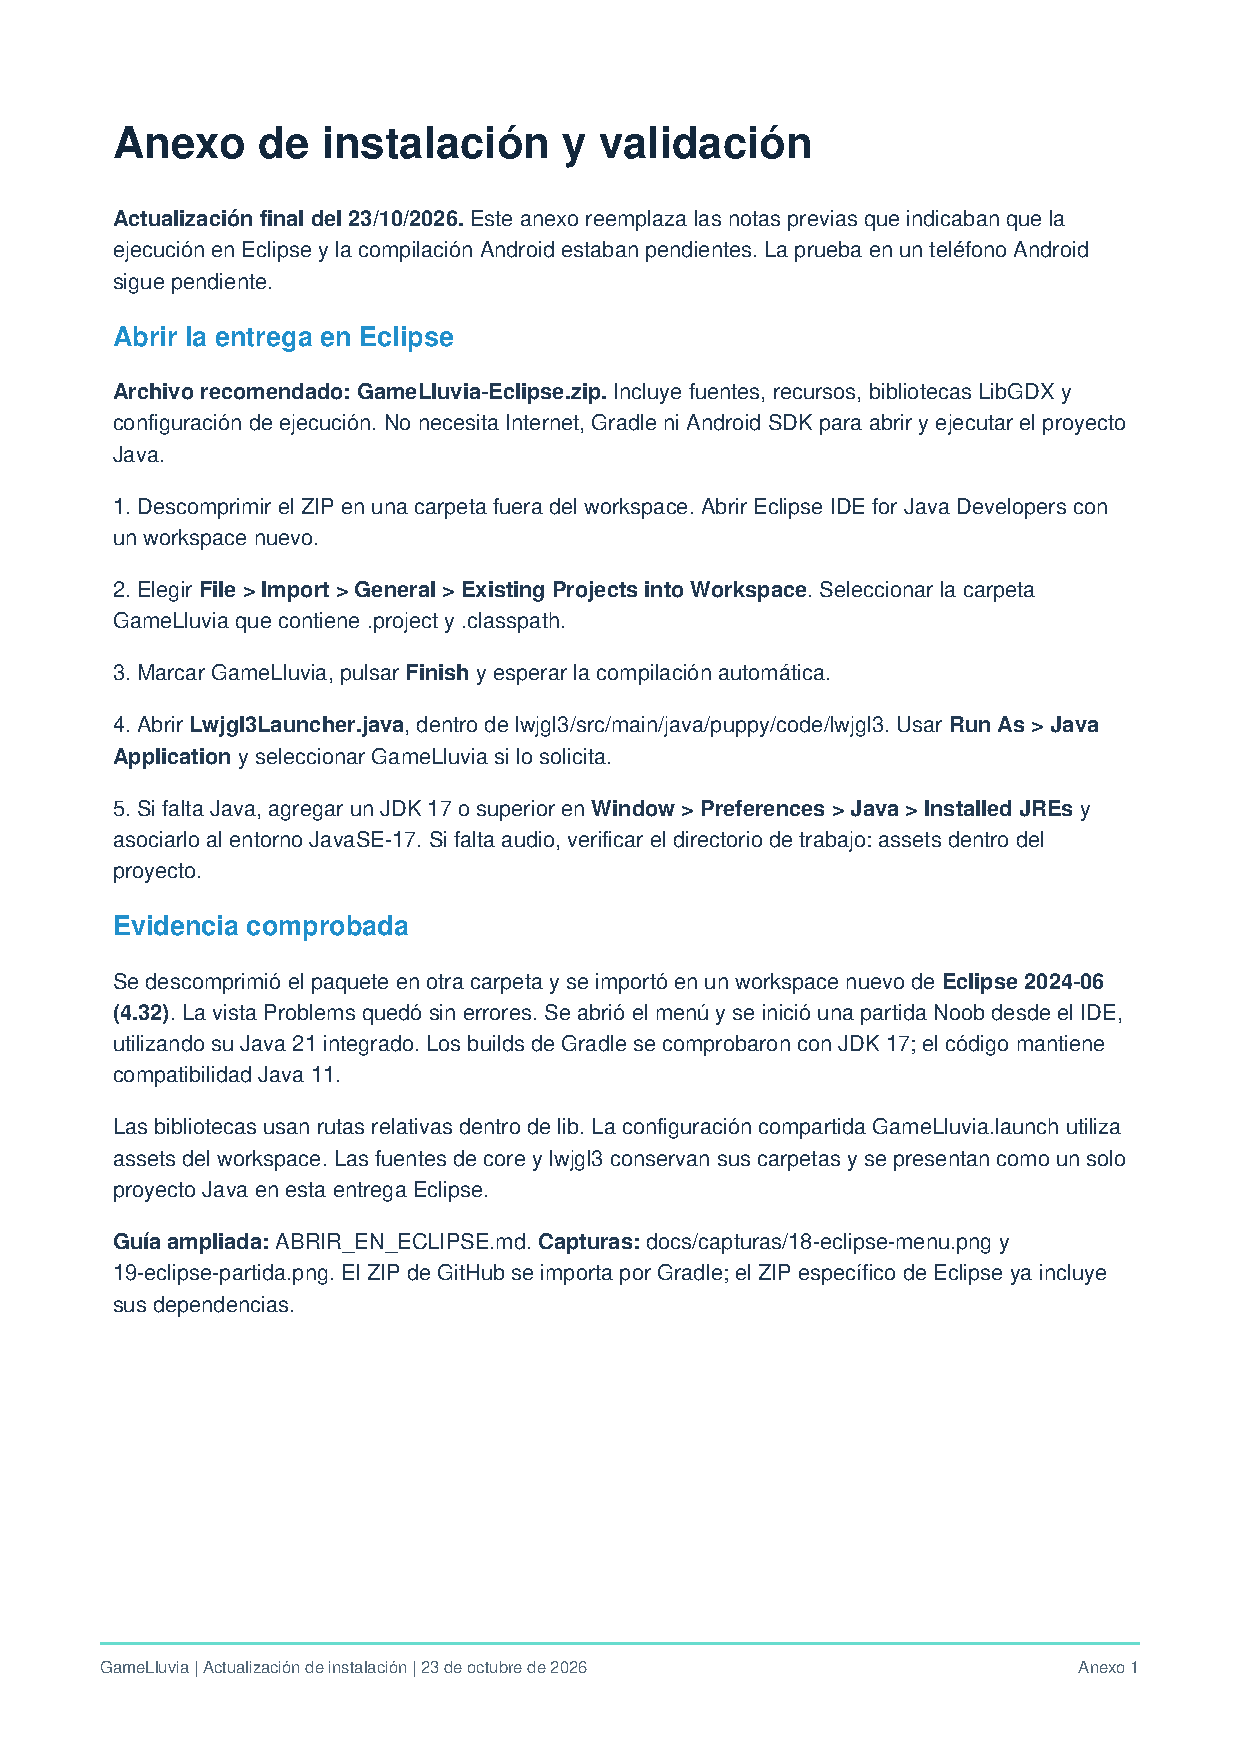
\includepdf[pages=-]{anexo-instalacion.pdf}
\end{document}

